In this Section we discuss how the \PARSEC{} applications are parallelized in Pthreads/OpenMP2.0 and how they can be implemented efficiently 
using a task-based approach.  When possible, we exploit dataflow relations in order to take advantage of implicit synchronization 
(as described in Section~\ref{sec:task-model}). If it is not possible we use conventional synchronization primitives such as locks,
atomics and barriers.

\paragraph{\textbf{Blackscholes}}
This application solves a Black-Scholes Partial Differential Equation~\cite{RePEc:ucp:jpolec:v:81:y:1973:i:3:p:637-54} to calculate the
prices for a portfolio of ten million European options.

\begin{figure}[t!]%
	\center
	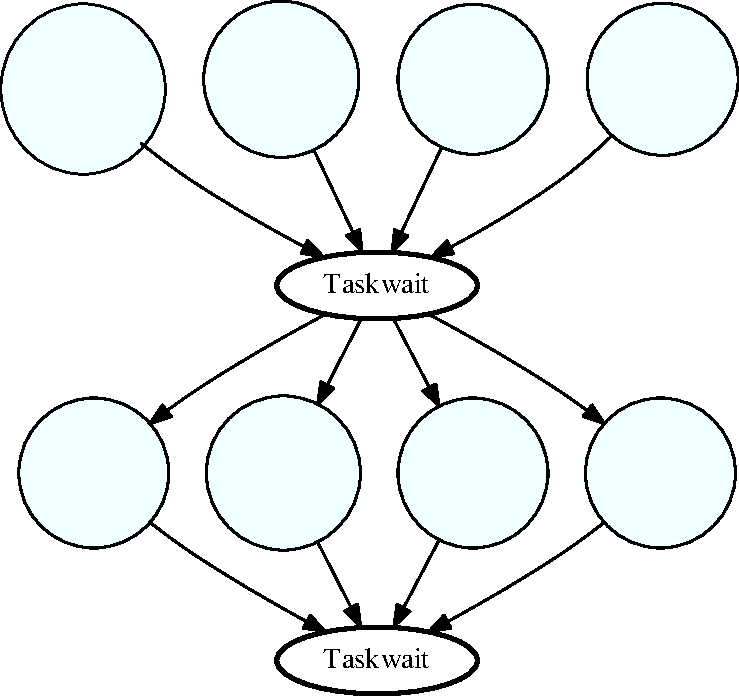
\includegraphics[width=0.5\columnwidth]{ifcg/figures/blackscholes_taskgraph}%
	\caption{Task-graph of blackscholes application.  No dependencies exit between tasks,
only barrier synchronization between iterations.}
	\label{fig:blackscholes_tg}%
	\vspace{.5cm}
\end{figure}

\paragraph{\textit{Pthreads}} This version simply divides the portfolio into
work units by the number of available threads, and stores them into the
\texttt{numOptions} array. Each thread calculates the prices for its
corresponding options and waits in a barrier until all the threads have
finished executing. The algorithm is run multiple times to obtain the final
estimation of the portfolio.


\paragraph{\textit{Task-based}} In the case of the task-based version, we
divide the work into units of a predefined block size. This block size allows
having much more task instances than threads, which implies a much better load
balance, as this is an embarrassingly parallel application with no dependencies
among tasks in the same run.  A task graph of the task-based implementation is
shown in figure \ref{fig:blackscholes_tg}.  We can see that this is an embarrassing
parallel application with only barrier synchronization between iterations of the 
main loop.  No data dependencies exist between tasks.
For all the task graphs shown in this document
we use smaller workloads than the ones used for evaluation.  This way it's easier
to read the task graphs.  For example in figure \ref{fig:blackscholes_tg} there are
four tasks per iteration, but this is easily configurable to hundreds or thousands 
of tasks.  Such is the case of the native workloads used for the evaluation of our 
implementations.



\begin{figure*}[ht!]
	\vspace{1cm}
	\centering
  \begin{subfigure}{0.9\textwidth}
		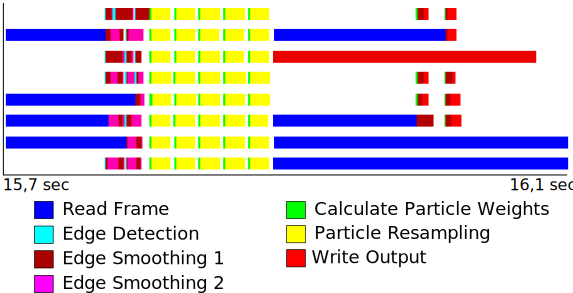
\includegraphics[width=\textwidth]{ifcg/figures/bodytrack-ompss-native-8-2dp_tasks_pthreads}
		\caption{Trivial Task-based Strategy}
	\label{fig:bodytrack-2dp_tasks-trace_pthreads}
  \end{subfigure}%
\\
\vspace{1cm}
\begin{subfigure}{0.9\textwidth}
		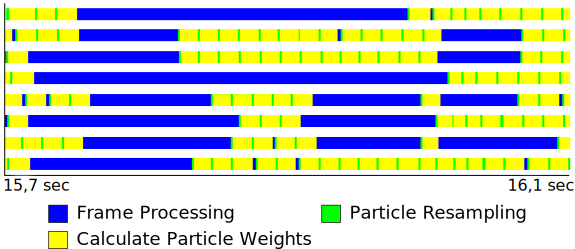
\includegraphics[width=\textwidth]{ifcg/figures/bodytrack-ompss-native-8-2dp_tasks_ompss}
		\caption{Optimal Task-based Strategy}
	\label{fig:bodytrack-2dp_tasks-trace_ompss}
  \end{subfigure}
	\caption{Parallel execution of Pthreads and task-based versions of \texttt{bodytrack} on an 8-core machine and native input size. Different parallel regions correspond to different colors.  White gaps in the figure, represent idle time.}%
	\label{fig:bodytrack-2dp_tasks-trace}%
\end{figure*}

\paragraph{\textbf{Bodytrack}}
Computer vision application that tracks a marker-less human body using multiple cameras
through an image sequence.  The application employs an annealed particle filter to track
the body using edges and the foreground silhouette as features of interest.

\begin{figure}[t!]%
	\center
	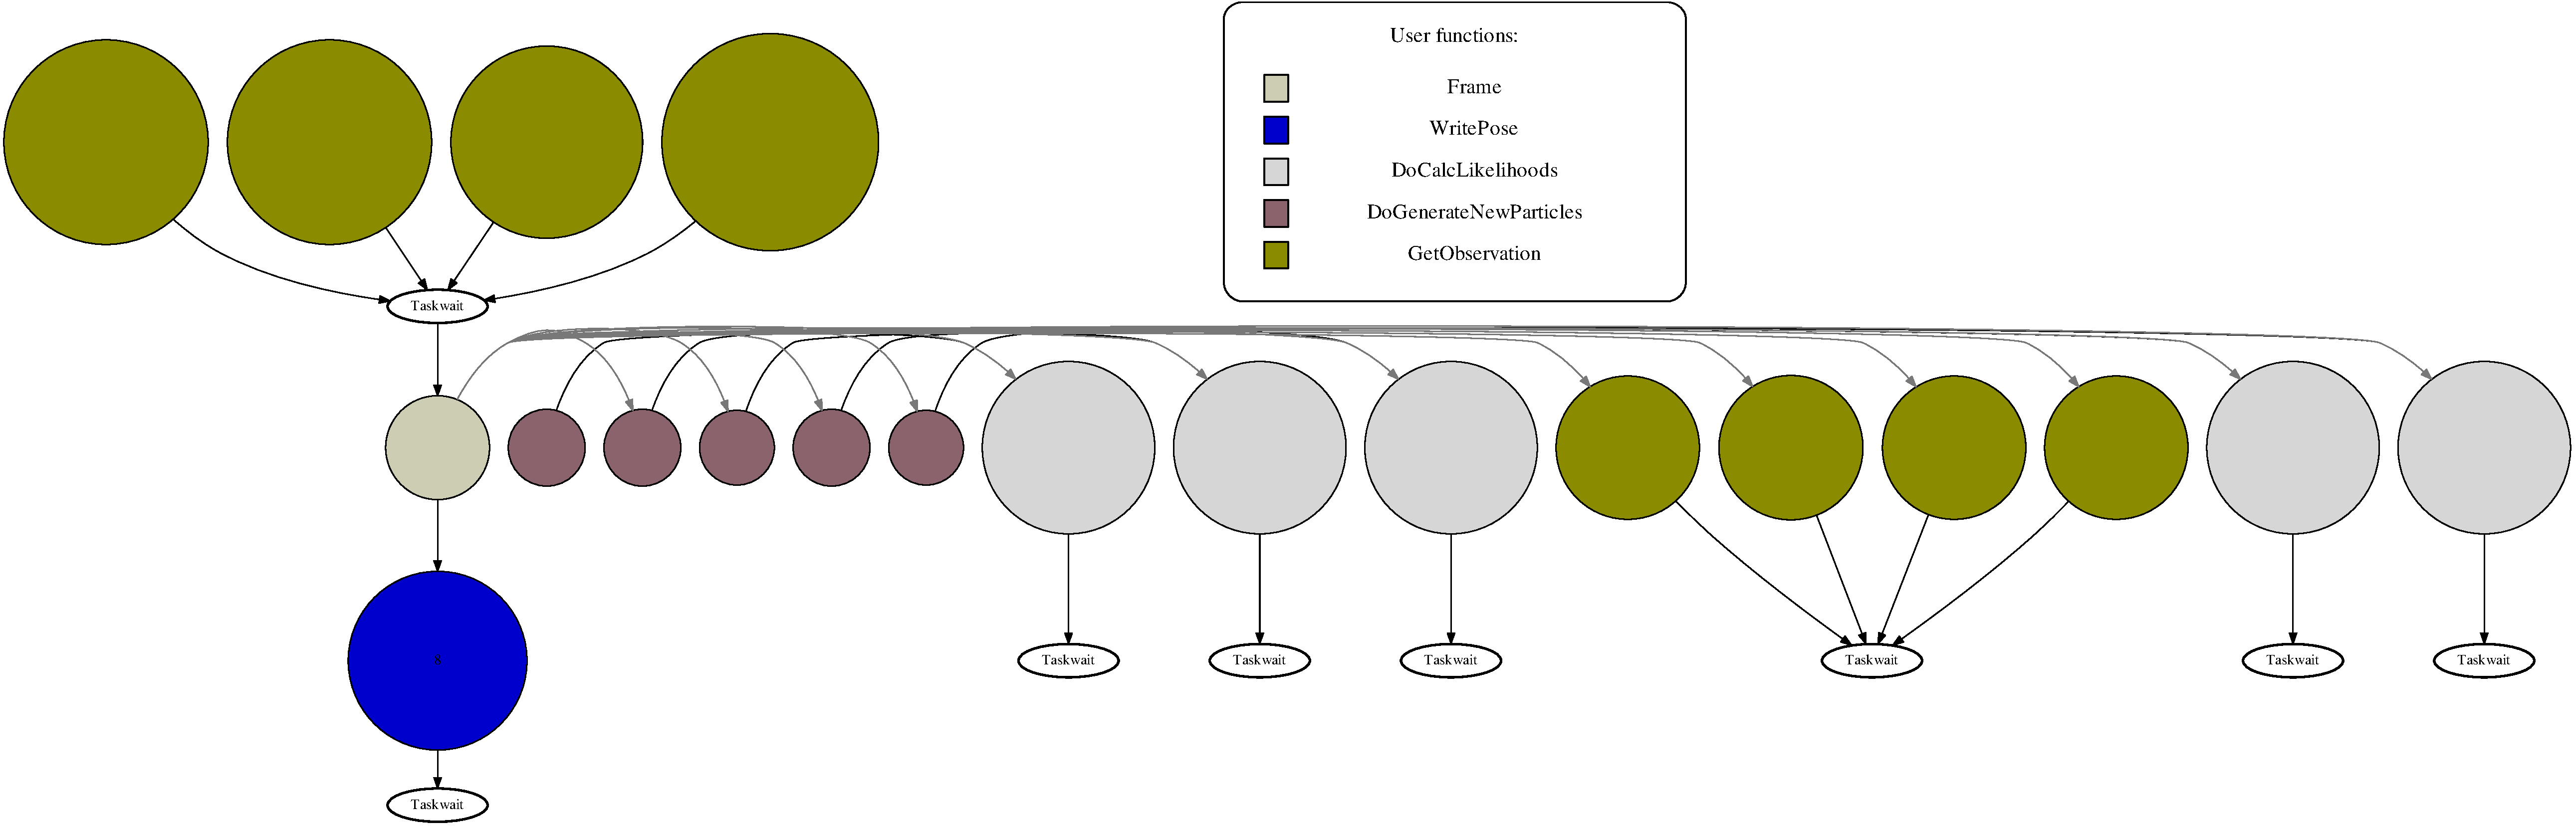
\includegraphics[width=\columnwidth]{ifcg/figures/bodytrack_taskgraph}%
	\caption{Task-graph of bodytrack application.  Edges show task data dependencies.}
	\label{fig:bodytrack_tg}%
	\vspace{.5cm}
\end{figure}



\paragraph{\textit{Pthreads}} \texttt{Bodytrack} applies the same algorithm on each frame
of the image sequence to track the different poses of the body.  The human body is modeled
as a tree-based structure, consisting of 7 conic cylinders.  It reads 4 images taken from
several cameras to capture a scene from 4 different angles, thus each frame consists of
these 4 images.  These images are read and encoded to a single data structure.  For each
frame, \texttt{bodytrack} extracts the edges and silhouette features for each of these 4
images.
In this feature extraction stage we have 3 different kernels.
\begin{enumerate}
	\item \textbf{Edge detection}: Gradient based edge detection.
	\item \textbf{Edge smoothing (phase 1)}: Gaussian filter used to smooth edges applied on array rows.
	\item \textbf{Edge smoothing (phase 2)}: Gaussian filter used to smooth edges applied on array columns.
\end{enumerate}
Afterwards, \texttt{bodytrack} goes through an annealed particle filter stage, which
consists of M annealing layers over a set of N particles.  The particles are multi-variate
configurations of the state and location of the tracked body.  Given the image features,
the particles are assigned weights, which increase or decrease the chance that a particle
represents a body part.  N particles are then chosen, depending on the probability
dictated by their weights.  Random noise is added to this set of particles, creating a new
set.  This process is repeated for all annealing layers. \texttt{Bodytrack} then picks one
of the M configurations, the one which has the highest weighted average.  This process has
two parallel kernels.
\begin{enumerate}[resume]
	\item \textbf{Calculate particle weights}: Computes weights for the particles, using the edges and silhouette produced from the previous stages.
	\item \textbf{Particle Resampling}: Adds Gaussian random noise to the particles, thus creating a new set of particles.
\end{enumerate}

In the case of Pthreads, the 4 images of a frame are read and processed in parallel using
one thread per image.  The Pthreads implantation is limited by the 4 images it can process
concurrently, while there is no other candidate work at this point.  A specific
asynchronous I/O implementation is required to read the files in parallel. Then, the
features extraction stage is executed using all the available threads, with a
synchronization barrier at the end of each phase. The same structure is followed in the
annealed particle filter stage, with two barriers at the end of each phase. Between the
two stages, serial code has to be executed, which leaves only one thread busy and the rest
idle.  Finally, the output results are written sequentially in one file.   


\paragraph{\textit{Task-based}} In the case of the task-based version, we adopt a more coarse grain approach. 
We do not parallelize the feature extraction stage, instead we 
taskify the whole frame processing, allowing concurrent execution of all frames. 
%Given enough frames to process, all threads can remain busy,
%which is not the case with the Pthreads version.
The parallel kernels of the annealed particle filter stage are taskified in our version, and synchronization is achieved
by dataflow annotations.  Figure \ref{fig:bodytrack_tg} shows a task graph of our implementation.  The directed edges show the
dependencies between the different tasks, which dictate the execution order of the tasks.
Each frame needs to be written when calculations are completed. In our version we can do this asynchronously while the threads are
busy with the processing stage of another frame.  Thus, output I/O is effectively overlapped with computation stages.


{Figure \ref{fig:bodytrack-2dp_tasks-trace} shows parallel executions of two different task-based implementations: 
The first one just mimics the Pthreads behavior (\ref{fig:bodytrack-2dp_tasks-trace_pthreads}) and the second is an optimal task-based implementation (\ref{fig:bodytrack-2dp_tasks-trace_ompss}).  
Different colored boxes represent different task types, as well the duration of that task type on each core. In both cases, the white gaps denote the time each thread spends idle.  
Both figures show the same duration for each execution. In the optimal version, all functionality is implemented within the frame-processing task, thus 
execution time for read-frame, edge-detection and edge-smoothing is represented with blue color (frame-processing).  
Tasks particle-resampling and calculate-particle-weights are also implemented as nested tasks. 
They are displayed with different colors (green and yellow respectively).  
We can observe that the Pthreads-like version suffers
from greater idle time compared to its optimal task-based counterpart. 
Work is distributed more efficiently in the optimal implementation
by processing different frames concurrently. 
This allows us to overlap I/O and serial code segments of one with available work from another one.
       
%To illustrate this point, Figure~\ref{fig:bodytrack-2dp_tasks-trace} shows an execution of \texttt{bodytrack} for two different frames. The x-axis represent time and the y-axis represent the cores where the execution takes place. 
%For example, a pixel of color blue in the (x,y) point means that at the instant x the core y is running the task codified by color blue. The red, dark red and green are tasks performing edge detection and edge smoothing, respectively.  
%The yellow color represents the task writing the output file. 
%Light green and magenta are the tasks that calculate particle weights and re-sample the particles. Light blue color annotates the idle time or sequential code execution. 
%%
%We can see how the task that writes the output file for frame N-1 (in yellow) is overlapped by the three first computation tasks of frame N, which does not happen in the Pthreads version of the code.
%This overlapping is the main source of performance gains archived by using the dataflow task-based paradigm with \texttt{bodytrack}. 
%Section~\ref{sec:evaluation} reports these improvements in detail.

\paragraph{\textbf{Canneal}}
This kernel uses a cache-aware simulated annealing~\cite{Banerjee:1994:PAV:185340} to
optimize routing cost of a chip design.  \texttt{Canneal} progressively swaps elements
that need to be placed in a large space, eventually converging to an optimal solution. The
problem is stored as a list with routing costs between nodes. 

\begin{figure}[t!]%
	\center
	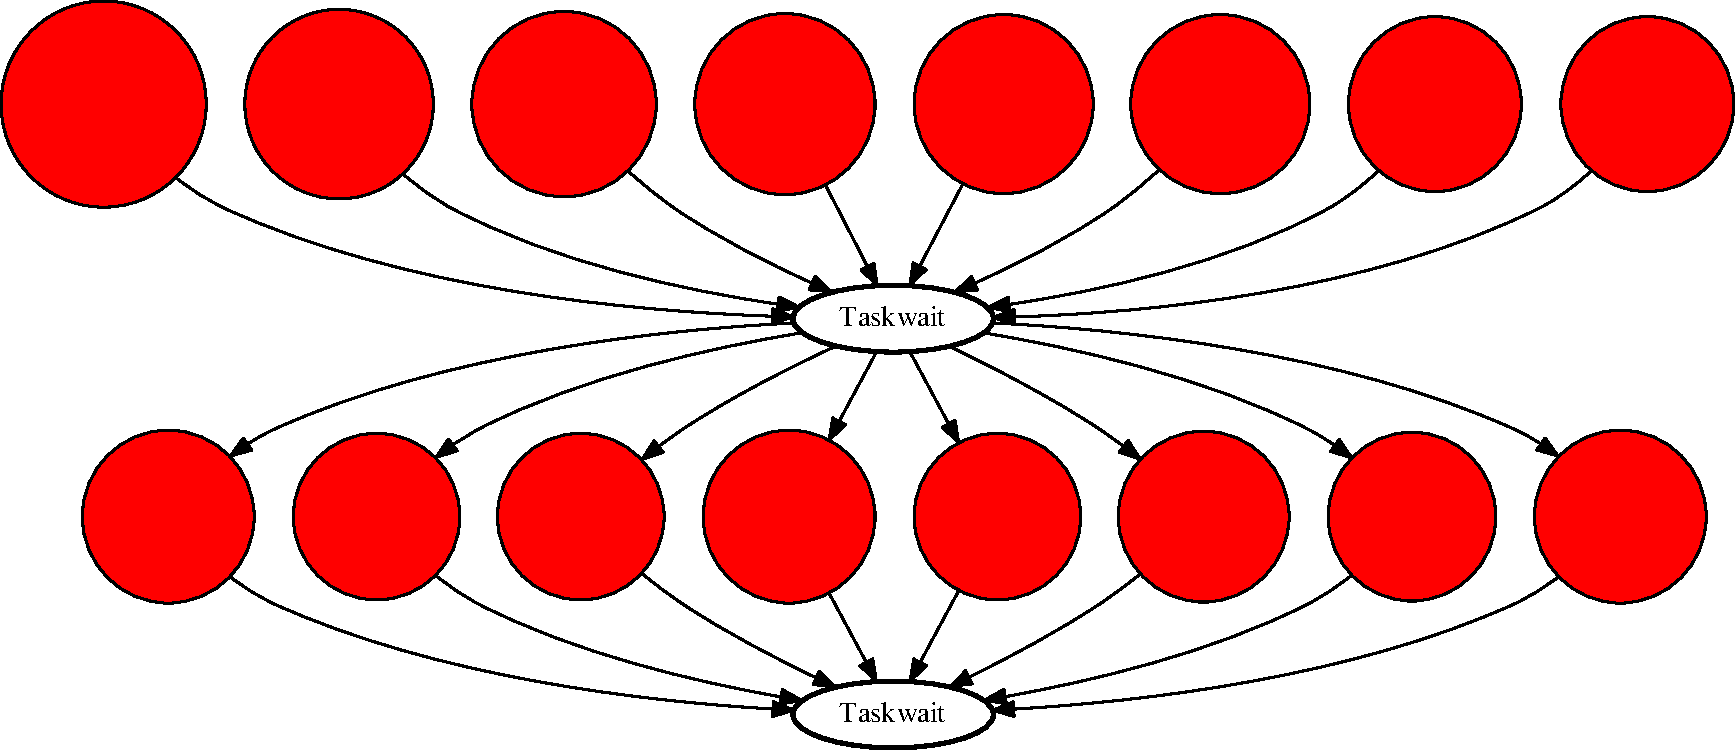
\includegraphics[width=.8\columnwidth]{ifcg/figures/canneal_taskgraph}%
	\caption{Task-graph of canneal application.  Only barrier synchronization among tasks.}
	\label{fig:canneal_tg}%
	\vspace{.5cm}
\end{figure}

\paragraph{\textit{Pthreads}} This version compares random element pairs of the graph
concurrently and swaps them until it converges to an optimal solution.  No locks are used
to protect the list from concurrent accesses/writes, but  swaps are done atomically
instead. However, the evaluation of the elements to be swapped is not atomic.  This means
that disadvantageous swaps may occur, which will require the algorithm to eventually swap
them again.  This method has provided better results than the alternative algorithm with
locks~\cite{bienia2008}.

\paragraph{\textit{Task-based}} Our task-based version follows the same paradigm.  Several
tasks are spawned without any dependencies between themselves. We use the same atomics as
with the Pthreads version.  Since tasks work with an arbitrary number of list elements, it
is not possible to describe which elements of the list a task is going to randomly access. 
In the task graph in figure \ref{fig:canneal_tg} it is clear that there are no data dependencies.
Synchronization is only achieved through the use of barriers.

We also try an alternative fine grain implementation, where a task is spawned for each
random pair of list elements.  This would allow the runtime to know if two tasks are
working on the same list of elements. However this implementation implied fine-grain
tasks. Each task would merely do a single swap between two list elements.  The overhead of
the dynamic scheduling is a problem in this scenario.  A more complex but more efficient
solution is suggested by Symeonidou et al.~\cite{Symeonidou:2013:DDR:2488551.2488558} with
the use of memory regions.  Adopting this method in a task-based model would allow the
programmer to describe parts of the list (or other pointer based data structures) and
express dataflow relations as abstract memory regions.  This solution also implies
fine-grain tasking and is not evaluated at the Symeonidou's work. 

\begin{figure}[t!]%
	\center
	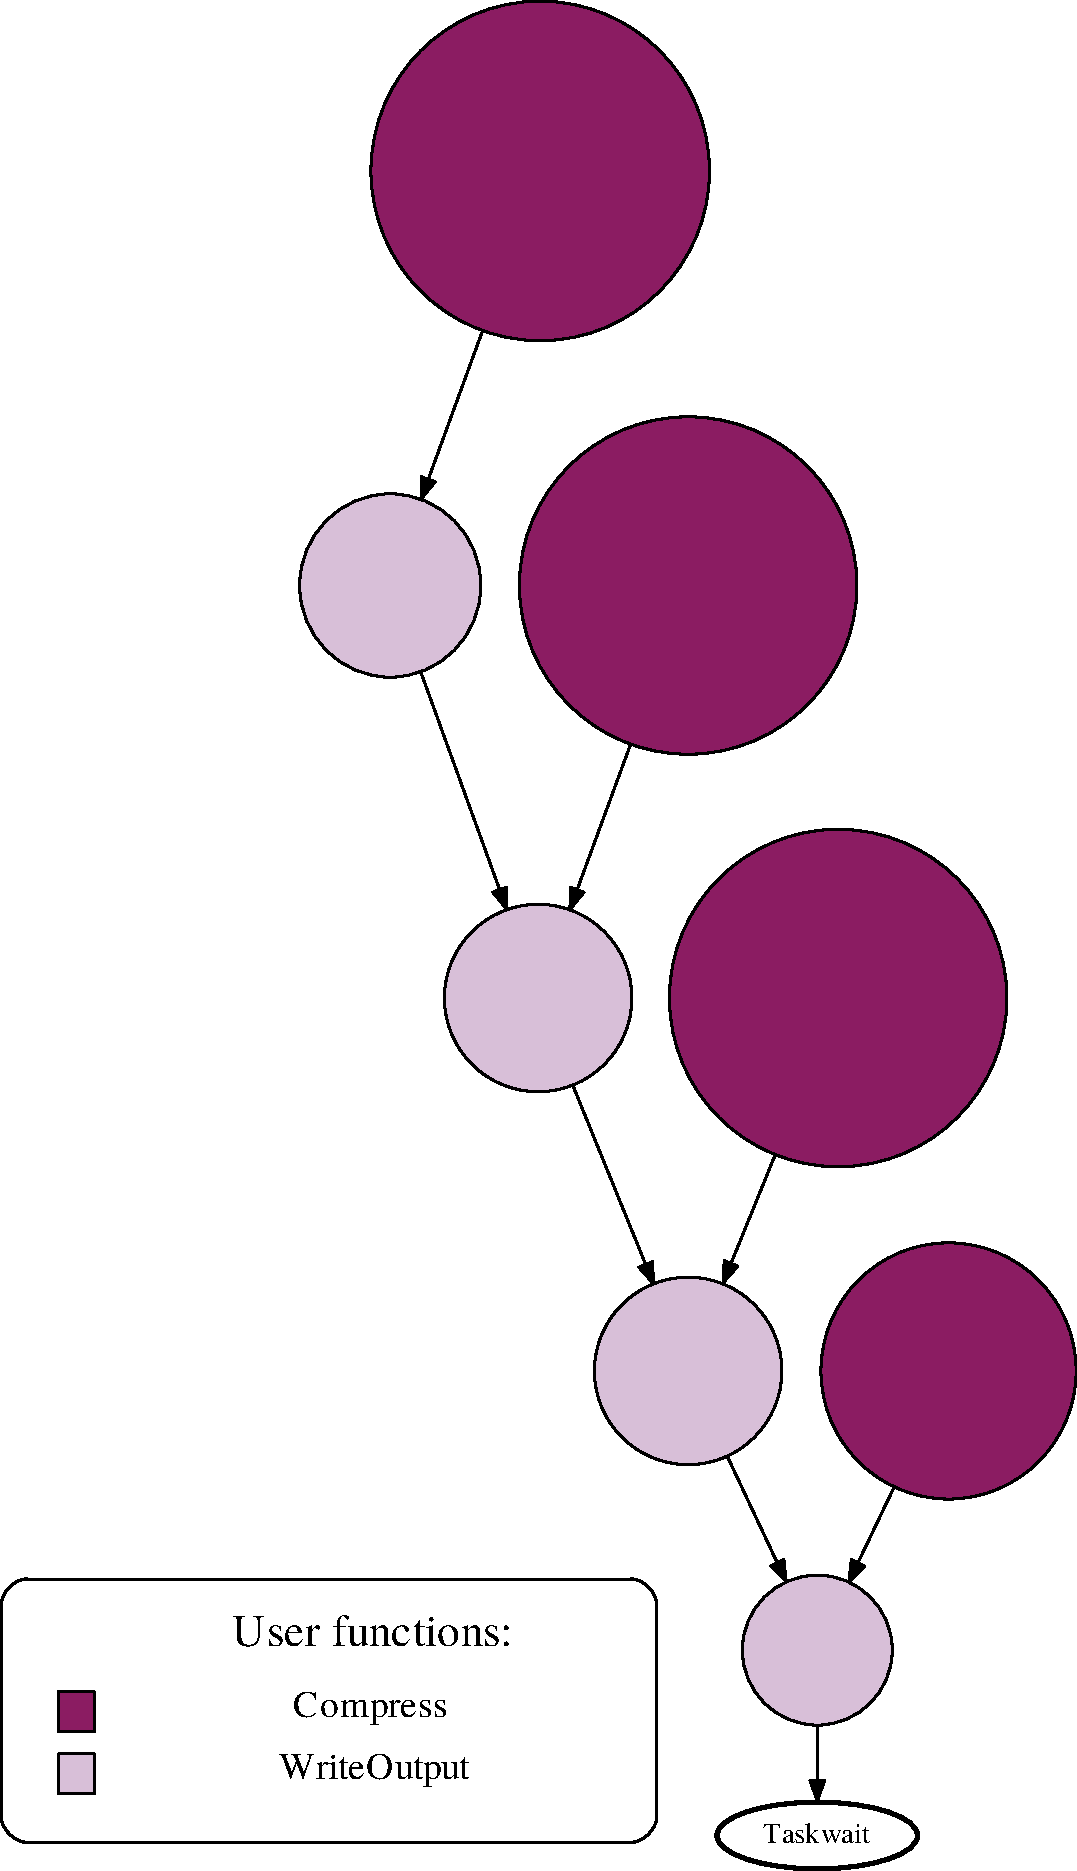
\includegraphics[width=.4\columnwidth]{ifcg/figures/dedup_taskgraph}%
	\caption{Task-graph of dedup application.  Data dependency edges force the correct order
of writting the data chunks to the output.}
	\label{fig:dedup_tg}%
	\vspace{.5cm}
\end{figure}


\paragraph{\textbf{Dedup}}
The \texttt{dedup} kernel is used to compress data streams using local and global
compression to achieve higher compression rates.  This method is called
deduplication~\cite{Quinlan:2002:ABP:1083323.1083333}.

\paragraph{\textit{Pthreads:}}
Dedup is parallelized using a pipeline model with the following stages:
\begin{itemize}
  \item \textbf{Fragment}:  First, the data-stream is read and partitioned at fixed positions into coarse grain data chunks. Each chunk can be processed individually by the rest of the stages. This stage is executed on a single thread.
  \item \textbf{Fragment Refine}:  A new data chunk initiates the second pipeline stage, where it is further partitioned into smaller fine-grain
	chunks.  The portioning is done by using the Rolling-fingerprint algorithm.  
  \item \textbf{Deduplication}:  This stage eliminates duplicate fine-grain chunks.  Unique chunks are stored in a hash-table.
	Locks are used here to protect	each bucket from concurrent accesses.
  \item \textbf{Compress}:  At this stage chunks are compressed in parallel.  Identical chunks are compressed only once as duplicates are removed 
	at the deduplication stage.
  \item \textbf{Reorder}:  This stage writes the final compressed output data to a file.  It writes only unique chunks' compressed data and for the
	duplicates it stores their hash values.  However this stage needs to reorder the data chunks as they are received
	to match the original order of the uncompressed data.
\end{itemize}

The Pthreads version maintains a queue and a thread pool dedicated to each stage.  When a
chunk becomes available at one stage, it is moved to the queue of the next stage.  Each
stage polls at its queue for available chunks to process. The reorder stage is done
sequentially with a devoted thread that can be in an idle loop waiting for previous stages
to finish.  Each thread pool  comprises by a number of threads equal to the number of
available cores.  The only exceptions are \texttt{Fragment} and \texttt{Reorder} stages,
which are served by a single thread each.

%\begin{figure}[ht!]%
%	\centering
%	\begin{lstlisting}
%void Fragment{
%  ...
%  while ( chunk = read_bytes() ) {
%		chunks[nCChunks][0] = chunk;
%		#pragma omp task inout(chunks[nCChunks]) 
%		Fragment(chunks[nCChunks]);
%		#pragma omp task inout(chunks[nCChunks])
%		WriteOutput(outfile, chunks[nCChunks]);
%		nCChunks++;
%		break;
%  }
%  #pragma omp taskwait
%	...
%}
%	\end{lstlisting}
%	\caption{Dedup task-based implementation pseudocode of the \texttt{Fragment} stage.}%
%	\label{lst:dedup-ompss}%
%\end{figure}

\begin{figure}[!t]%
	\centering
	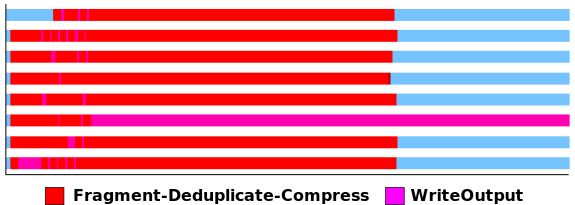
\includegraphics[width=0.9\columnwidth]{ifcg/figures/dedup-ompss-native-8-2dp_tasks}%
	\caption{Parallel execution of the task-based version of \texttt{dedup} on an 8-core machine and native input size. Different task types correspond to different colors.}%
	\label{fig:dedup-2dp_tasks-trace}%
	\vspace{.5cm}
\end{figure}


\paragraph{\textit{Task-based}}
In our implementation we taskify each pipeline stage and express data dependencies using static arrays and dataflow relations, one for each pipeline stage.
\texttt{FragmentRefine} however partitions the data chunks into very fine grain segments, ranging from a few hundreds to thousands. For such granularity,
our approach suffers from high overheads due to dynamic schedulnig overhead. 
The same is observed in~\cite{Vandierendonck:2013:DSP:2503210.2503233}, where 
an alternative approach is adopted. In their approach, two pipelines are identified: The outer pipeline, consisting of stages \texttt{Fragment}, \texttt{InnerPipeline}
and \texttt{Reorder}. The inner pipeline consists of \texttt{FragmentRefine}, \texttt{Deduplicate} and \texttt{Compress}.  To reduce the dynamic scheduling overhead,
they merge together \texttt{Deduplicate} and \texttt{Compress}. By doing so, the available parallelism is limited, but still there is enough work not to harm performance
and scalability. In our approach, we merge together the inner pipeline, creating one sequential function, exploiting only the parallelism available in the outer pipeline.
Even in this scenario, the available parallelism is still abundant, since the application is bound by the writing of the output file, which is sequential.  
Figure~\ref{fig:dedup-2dp_tasks-trace} shows a trace of the task-based version.  We can see that communication stage (in yellow) is effectively overlapped with the computation stage (in red), however,
there is not enough work to keep all the threads finish, until the end of the execution.

Furthermore, we modify the \texttt{Reorder} stage, by replacing it with a simple stage where the chunk is simply written to file (\texttt{WriteOutput}).
Using dataflow relations and a shared output resource between the \texttt{WriteOutput} tasks, we ensure that chunk \texttt{N-1} will be written before chunk \texttt{N}. 
Thus, we do not need to reorder data chunks in this task type.  Moreover, the scheduler makes sure chunks are written as soon as they become available by the \texttt{InnerPipeline} task, an improvement
over the Pthreads version, where \texttt{Reorder} instances need to idle wait until all previous chunks ones have been written.  
Figure \ref{fig:dedup_tg} shows the dependencies among tasks.  We can observe that \texttt{WriteOutput} tasks will be run in the correct
order, as soon as their dependencies are resolved.
Another difference between the two versions, is that Pthreads 
oversubscribe threads to cores for each pipeline stage, while in our implementation we only assign one thread to each core.


\paragraph{\textbf{Facesim}}
Computes a visually realistic human face animation by simulating the underlying physics.  As input it uses a 3D model of a human face 
containing both a tetrahedra mesh and triangulated surfaces for the flesh and bones, respectively. Additionally it uses 
a time sequence of muscle movement \cite{Sifakis:2005:ADF:1073204.1073208}.

\paragraph{\textit{Pthreads}}
The application statically decomposes the original tetrahedron mesh into smaller partitions, equal to the number of available threads.
%The boundaries of the partitions are replicated to avoid synchronization. The trade-off is redundant computations. For the bones, they 
%are employed serially. 
There are three main parallel kernels:
\begin{itemize}
  \item \textbf{Update State}: Calculates the steady properties of the mesh, constrains like stress and stiffness.  
%This is done by solving a nonlinear system of equationsusing the Newton-Rhapson method.  
  \item \textbf{Add Forces}: Computes the force contribution between vertices acting on the 3D model.
  \item \textbf{Conjugate Gradient (CG)}:  An iterative method that solves the linear system produced by the 
other two previous kernels and find the final displacement of the vertices for the current frame.
\end{itemize}

\texttt{Update\_State} and \texttt{Add\_Forces} kernels consist of one and two parallel loops respectively, while \texttt{CG} has three. 
Synchronization between loops and kernels is achieved by barriers.  The corresponding force computations from the skeleton are also done 
in \texttt{Update\_State} and \texttt{Add\_Forces}, but after the parallel computations on the tetrahedra mesh have been made. 
In Pthreads a master thread is assigning work to all threads in a round-robin fashion through a queuing system.  Each thread maintains 
its private queue, which is protected by locks.

%\begin{figure}[!t]%
%	\centering
%	\includegraphics[width=0.8\columnwidth]{figures/facesim-ompss-native-8-2dp_tasks}%
%	\caption{Parallel execution of the task-based version of \texttt{facesim} on an 8-core machine while simulating a frame. 
%	Different task types correspond to different colors, while idle time is represented in light blue color.}%
%	\label{fig:facesim-2dp_tasks-trace}%
%\end{figure}

\paragraph{\textit{Task-based}}
In the task-based version, the application level queuing system is completely replaced by the OmpSs runtime.  In our initial implementation 
all parallel loops are taskified. 
Additionally,  in \texttt{Update\_State} there is a sequential code segment, 
\texttt{Update\_Collision\_Penalty\_Forces}.  
This code segment operates on the bones, while the parallel loop of \texttt{Update State} does so on the tetrahedra.  
By taskifying it and adding dataflow relations between this Section and the following \texttt{Add\_Forces} kernel, we can overlap 
\texttt{Update\_Collision\_Penalty\_Forces} with the rest of \texttt{Update\_State}.


%\edit{In the \texttt{CG} kernel, we managed to remove two out of three barriers, which synchronized the different parallel loops, by using dataflow relations 
%to describe data dependencies.  One barrier could not be removed as it protects the residual calculation at theend of each iteration of the solver, 
%whose value is used to control whether we exit the loop or not.}  
%\edit{This initial implementation suffered from high task creation time in the \texttt{CG} kernel.  Note that this is an issue of OmpSs' runtime, out OpenMP 4.0 task implementation 
%did not manifest this issue.}
To improve performance we refactor tasks' creation in \texttt{CG} by nesting the first task creation loop inside another task.
This enables us to overlap task creation time with computation, which contributes to increase \texttt{Facesim's} task-based implementation performance.  
Although we achieve better scalability than the original code, task creation still imposed overheads. To address this issue
we replace tasks in \texttt{CG} with the OmpSs parallel loops construct (equivalent to the OpenMP one), which implements loop worksharing 
with a task. Even though this approach limits the available parallelism (barrier synchronization, no dataflow annotations), the overhead 
associated to task creation and scheduling is greatly reduced and overall performance improved.

\paragraph{\textbf{Ferret}}
Content similarity search server for feature-rich data~\cite{Lv:2006:FTC:1218063.1217966} like audio, video, images, etc.
The benchmark application is configured for image similarity search.  
%\begin{figure}[t!]%
%	\begin{lstlisting}
%void load() {
%	int i = 0;
%	while( load_image(image[i]) ) {
%		#pragma omp task in(image[i]) out(seg_images[i])
%		seg_images[i] = t_seg(image[i]);
%		#pragma omp task in(seg_images[i]) out(extract_data[i])
%		extract_data[i] = t_extract(seg_images[i]);
%		#pragma omp task in(extract_data[i]) out(vectoriz_data[i])
%		vectoriz_data[i] = t_vec(extract_data[i]);
%		#pragma omp task in(vectoriz_data[i]) out(rank_results[i])
%		rank_results[i] = t_rank(vectoriz_data[i]);
%		#pragma omp task in(rank_data[i]) out(outstream)
%		t_out(rank_data[i], outstream);
%		i++;
%	}
%	#pragma omp taskwait
%}
%	\end{lstlisting}
%	\caption{Ferret ompss implementation}%
%	\label{lst:ferret-ompss}%
%\end{figure}

\begin{figure}[t!]%
	\center
	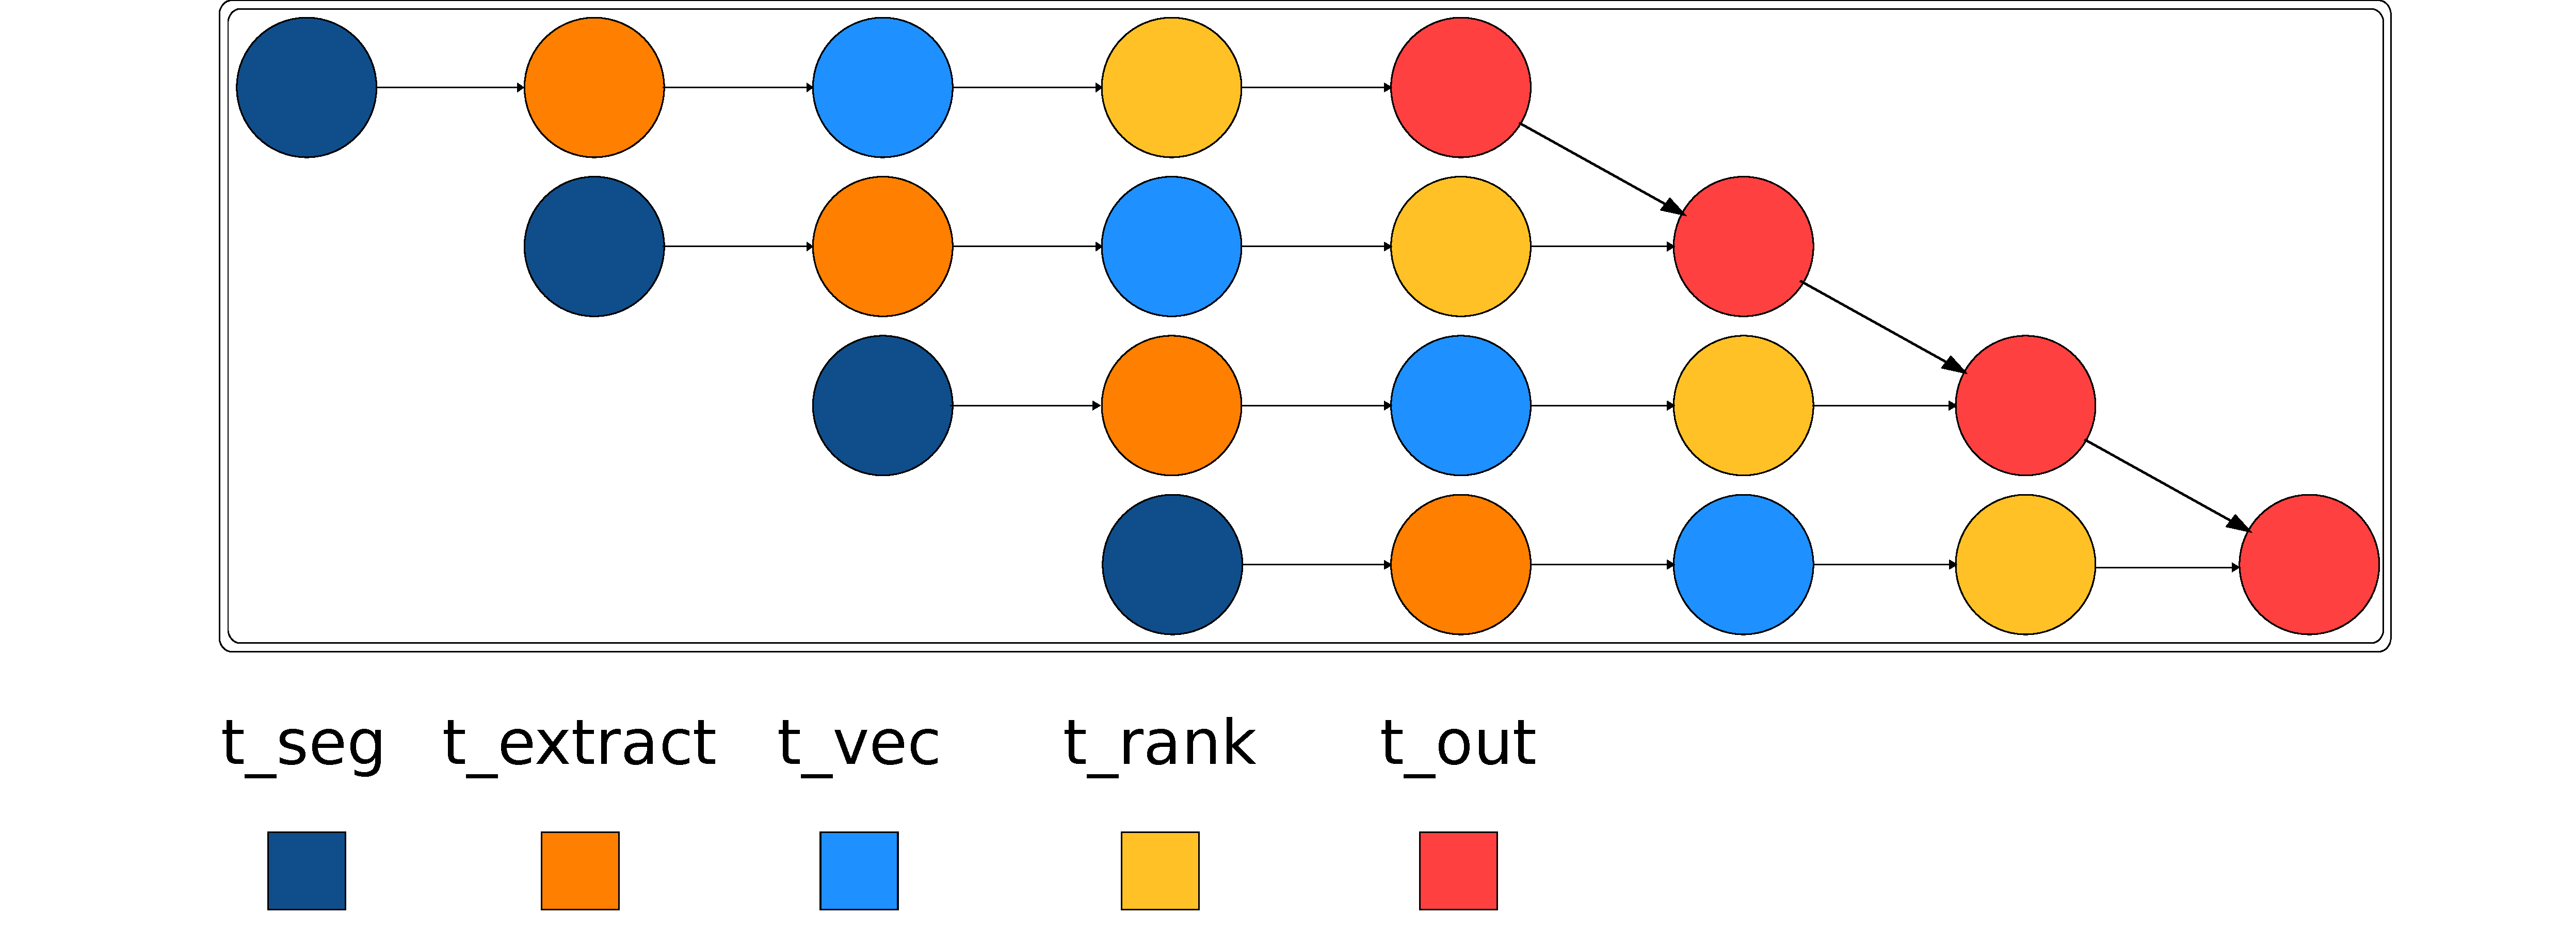
\includegraphics[width=0.9\columnwidth]{ifcg/figures/ferret_tg}%
	\caption{Task-graph of ferret showing the pipelined execution model.  Edges show data dependencies among different tasks.}
	\label{fig:ferret_tg}%
	\vspace{.5cm}
\end{figure}

\paragraph{\textit{Pthreads}}
Ferret is parallelized using a pipeline model.  A serial query is broken down into 
6 pipeline stages:
\begin{itemize}
  \item \textbf{Load}:  This stage loads an image that is going to be used as a query.
  \item \textbf{Segmentation}:  At this stage the image is decomposed into the different objects displayed on it.
	Different weight vectors are to be assigned on each object to achieve better results.
%	For example if an object is identified as a background it will have a smaller weight
%	than other objects.
  \item \textbf{Extract}:  At this stage a 14-dimensional vector is computed for each object from the segmentation stage, 
														describing features such as color, area, state, etc.
  \item \textbf{Vectorization}:  This is the indexing stage that tries to find a set of candidate images in the database.
  \item \textbf{Rank}:  This stage ranks the results found, using the EMD metric for each query-object's vector
	and the database's image vectors.
  \item \textbf{Output}:  Outputs the result of the ranking stage.  Multiple instances of
	this stage need to run serially, since they all share the same output stream.

\end{itemize}

In the Pthreads version every stage is served by a dedicated thread-pool of N threads each, where N is the number of available cores.
The only exceptions are the \texttt{Load} and \texttt{Output} stages that are executed by a respective single thread.
Each stage polls on its corresponding queue for available work.  When a stage finishes,
it pushes the results to the next stage's queue. 

\paragraph{\textit{Task-based}}
In this version, we implement a variation of this pipeline model. As soon as the first
stage, \texttt{Load}, finds a new image, it spawns all stages of a pipeline for that
image, thus reducing the pipeline to five stages.  We model the dataflow relations between
different stages as simple one dimension arrays, as shown in
Figure~\ref{lst:ferret-ompss}.  Tasks working on different image queries do not share any
dependencies. An exception is task \texttt{t\_out} which shares the same output file
between all pipelines, thus sequential execution is forced between all instances of this
task.  The pipeline stages and dependencies are constructed a priori, which is good enough
for this application, but this is not always the case.
\cite{Lee:2013:OPP:2486159.2486174} proposes a system that can handle dynamic pipeline
creation by constructing a DAG with the stages using indexes and the
\texttt{cilk\_continue} and \texttt{cilk\_wait} keywords.  Indexes are used to define the
different pipeline stages, while \texttt{cilk\_continue} creates a stage that can run once
all previous stages in the same pipeline iteration are done, and \texttt{cilk\_wait}
creates a stage that will wait for its stage counterpart of the previous iteration to
finish.  A strategy based on versioning the dependency objects between the stages has been
proposed~\cite{Vandierendonck:2011:PPG:2001252.2001265}.  Output dependencies are renamed
and privatized, thus the static array for privatization is not required.  

Figure \ref{fig:ferret_tg} shows the task-graph of the \texttt{ferret} application.
Colored nodes denote the concurrent tasks (each color matches a specific task type).
Tasks that have data dependencies are connected by directed edges.  By inspecting the
task-graph we can see a pipeline pattern of execution.  Despite the fact that the
task-based approach does not significantly improve the overall performance, as we can see
in Section~\ref{sec:task_bench_evaluation}, it significantly reduces the effort required
to express the pipeline parallelism, compared its Pthreads counterpart, as it is shown in
Section~\ref{sec:lines} in detail.


\paragraph{\textbf{Fluidanimate}}
This application simulates incompressible fluid interactive animation, using the 
Smoothed Particle Hydrodynamics (SPH) method~\cite{Muller:2003:PFS:846276.846298}.

\begin{figure}[t!]%
	\center
	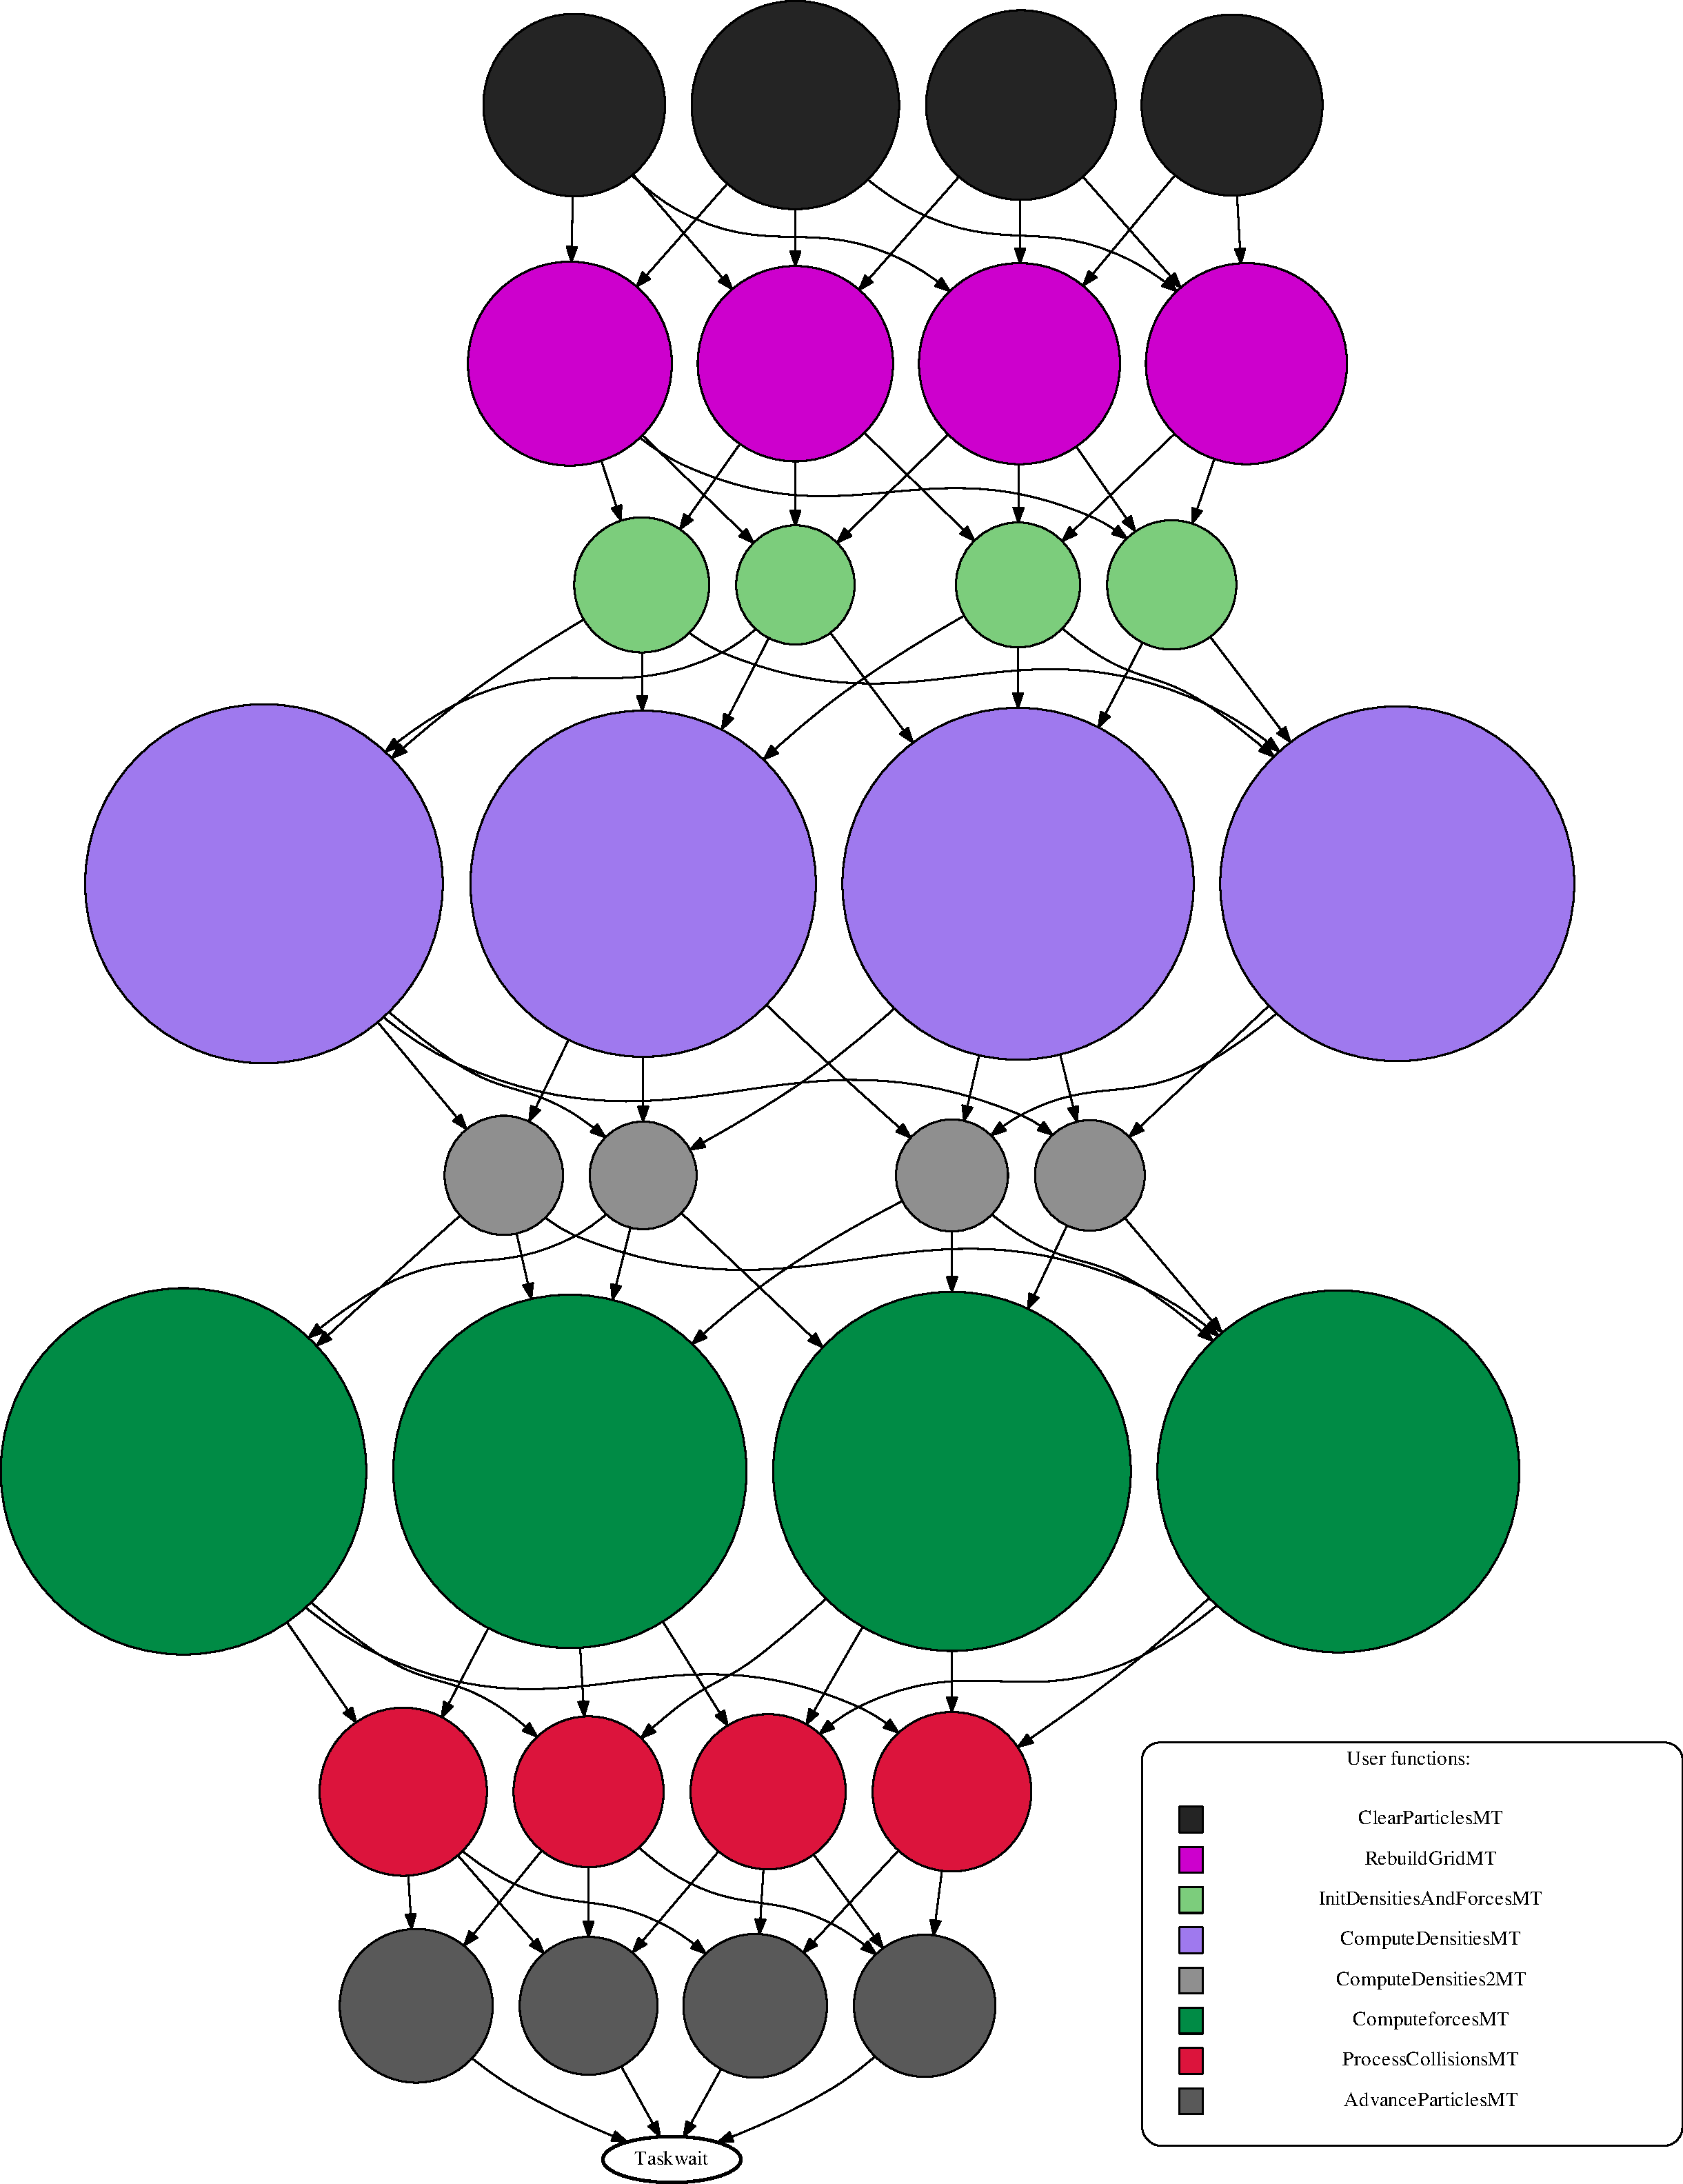
\includegraphics[width=.6\columnwidth]{ifcg/figures/fluidanimate_taskgraph}%
	\caption{Task-graph of fluidanimate application. Edges represent data dependencies among
tasks}
	\label{fig:fluidanimate_tg}%
	\vspace{.5cm}
\end{figure}

\paragraph{\textit{Pthreads}}
\texttt{Fluidanimate} uses five special kernels which are responsible for rebuilding the
spatial index, computing fluid densities and forces at given points, handling fluid
collisions with the scene geometry and finally updating particle locations The fluid
surface is partitioned and each thread works on its own grid segment.  The kernels are
parallelized as do-all loops, separated by barriers. Moreover, there are cases where these
threads need to update values beyond their partition, which are handled using locks.

\paragraph{\textit{Task-based}}
The task-based implementation follows the same approach, we apply a loop tiling
transformation, for each parallel loop, and taskified each iteration.  
Figure \ref{fig:fluidanimate_tg} show how dependencies form among between tasks.  
Tasks from different loops can run concurrently, as soon as their dependencies are met.
For example we see that the first task of each loop, only requires that the first two tasks
from the previous loop finish their execution to have their dependencies resolved.
We maintain the
same barrier and lock synchronization scheme, using the OmpSs synchronization primitives.

\begin{figure}[t!]%
	\center
	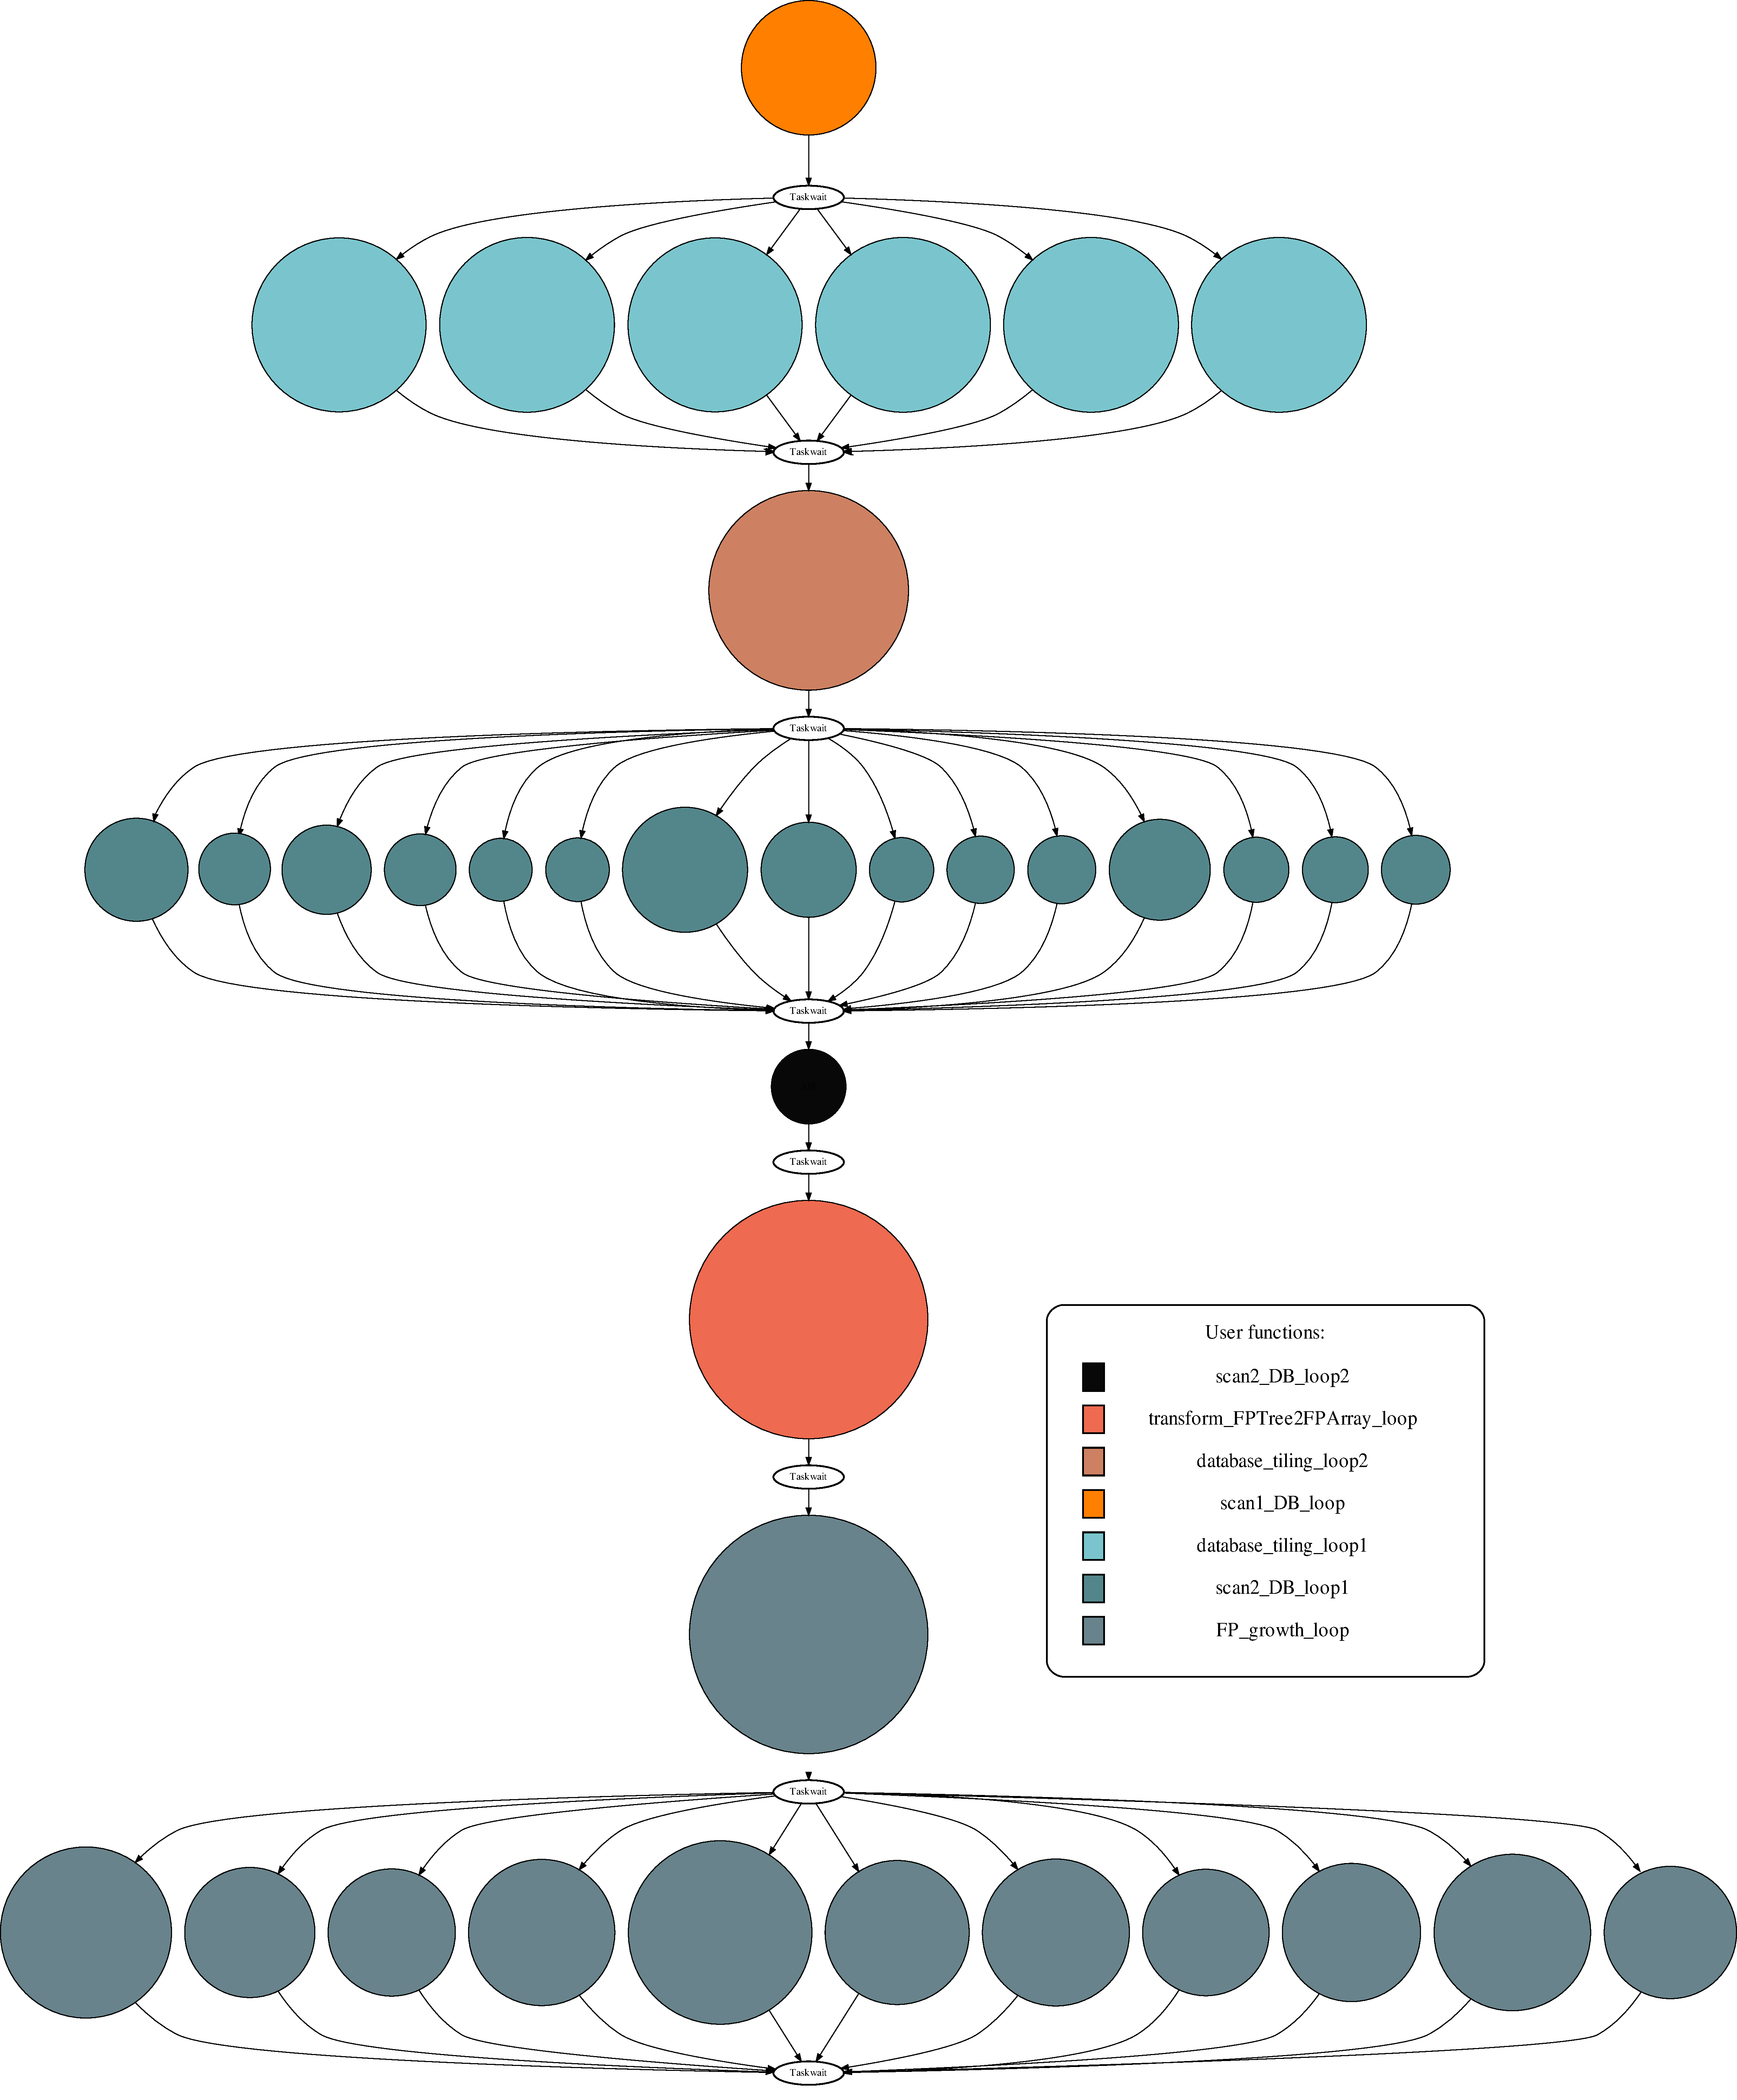
\includegraphics[width=.8\columnwidth]{ifcg/figures/freqmine_taskgraph}%
	\caption{Task-graph of freqmine application.  Edges represent data dependencies among
tasks.}
	\label{fig:freqmine_tg}%
	\vspace{.5cm}
\end{figure}

\paragraph{\textbf{Freqmine}}
Data mining application that makes use of an array-based version of the Frequent Pattern
(FP) growth method for Frequent Itemset Mining~\cite{conf/fimi/GrahneZ03}.

\paragraph{\textit{Pthreads}}
The application uses a compact tree data structure, denoted \emph{FP-tree}~\cite{Han:2000:MFP:335191.335372}, to store information about frequent patterns of the transaction database.  The FP-tree is coupled with a header table, which is a list of database items, sorted by decreasing order of occurrences.
The FP-growth algorithm traverses the FP-tree structure recursively, constructing new FP-trees until the complete set of frequent itemsets is generated.
There are three parallel kernels.  The \texttt{Build\_FP-tree\_header\_table} kernel performs a database scan 
and counts the number of occurrences of each item.  The result is the FP-tree header table.   
\texttt{Build\_Prefix\_tree} kernel performs a second database scan required to build the prefix tree
and the \texttt{Data\_Mining} kernel obtains the frequent itemset information by using the previous two structures.  It creates
an additional lookup table, which allows faster traversals on sparse itemsets.
The original \PARSEC{} benchmark uses OpenMP2.0 for loop parallelization inside each kernel.  

\begin{figure}[ht!]%
	\center
	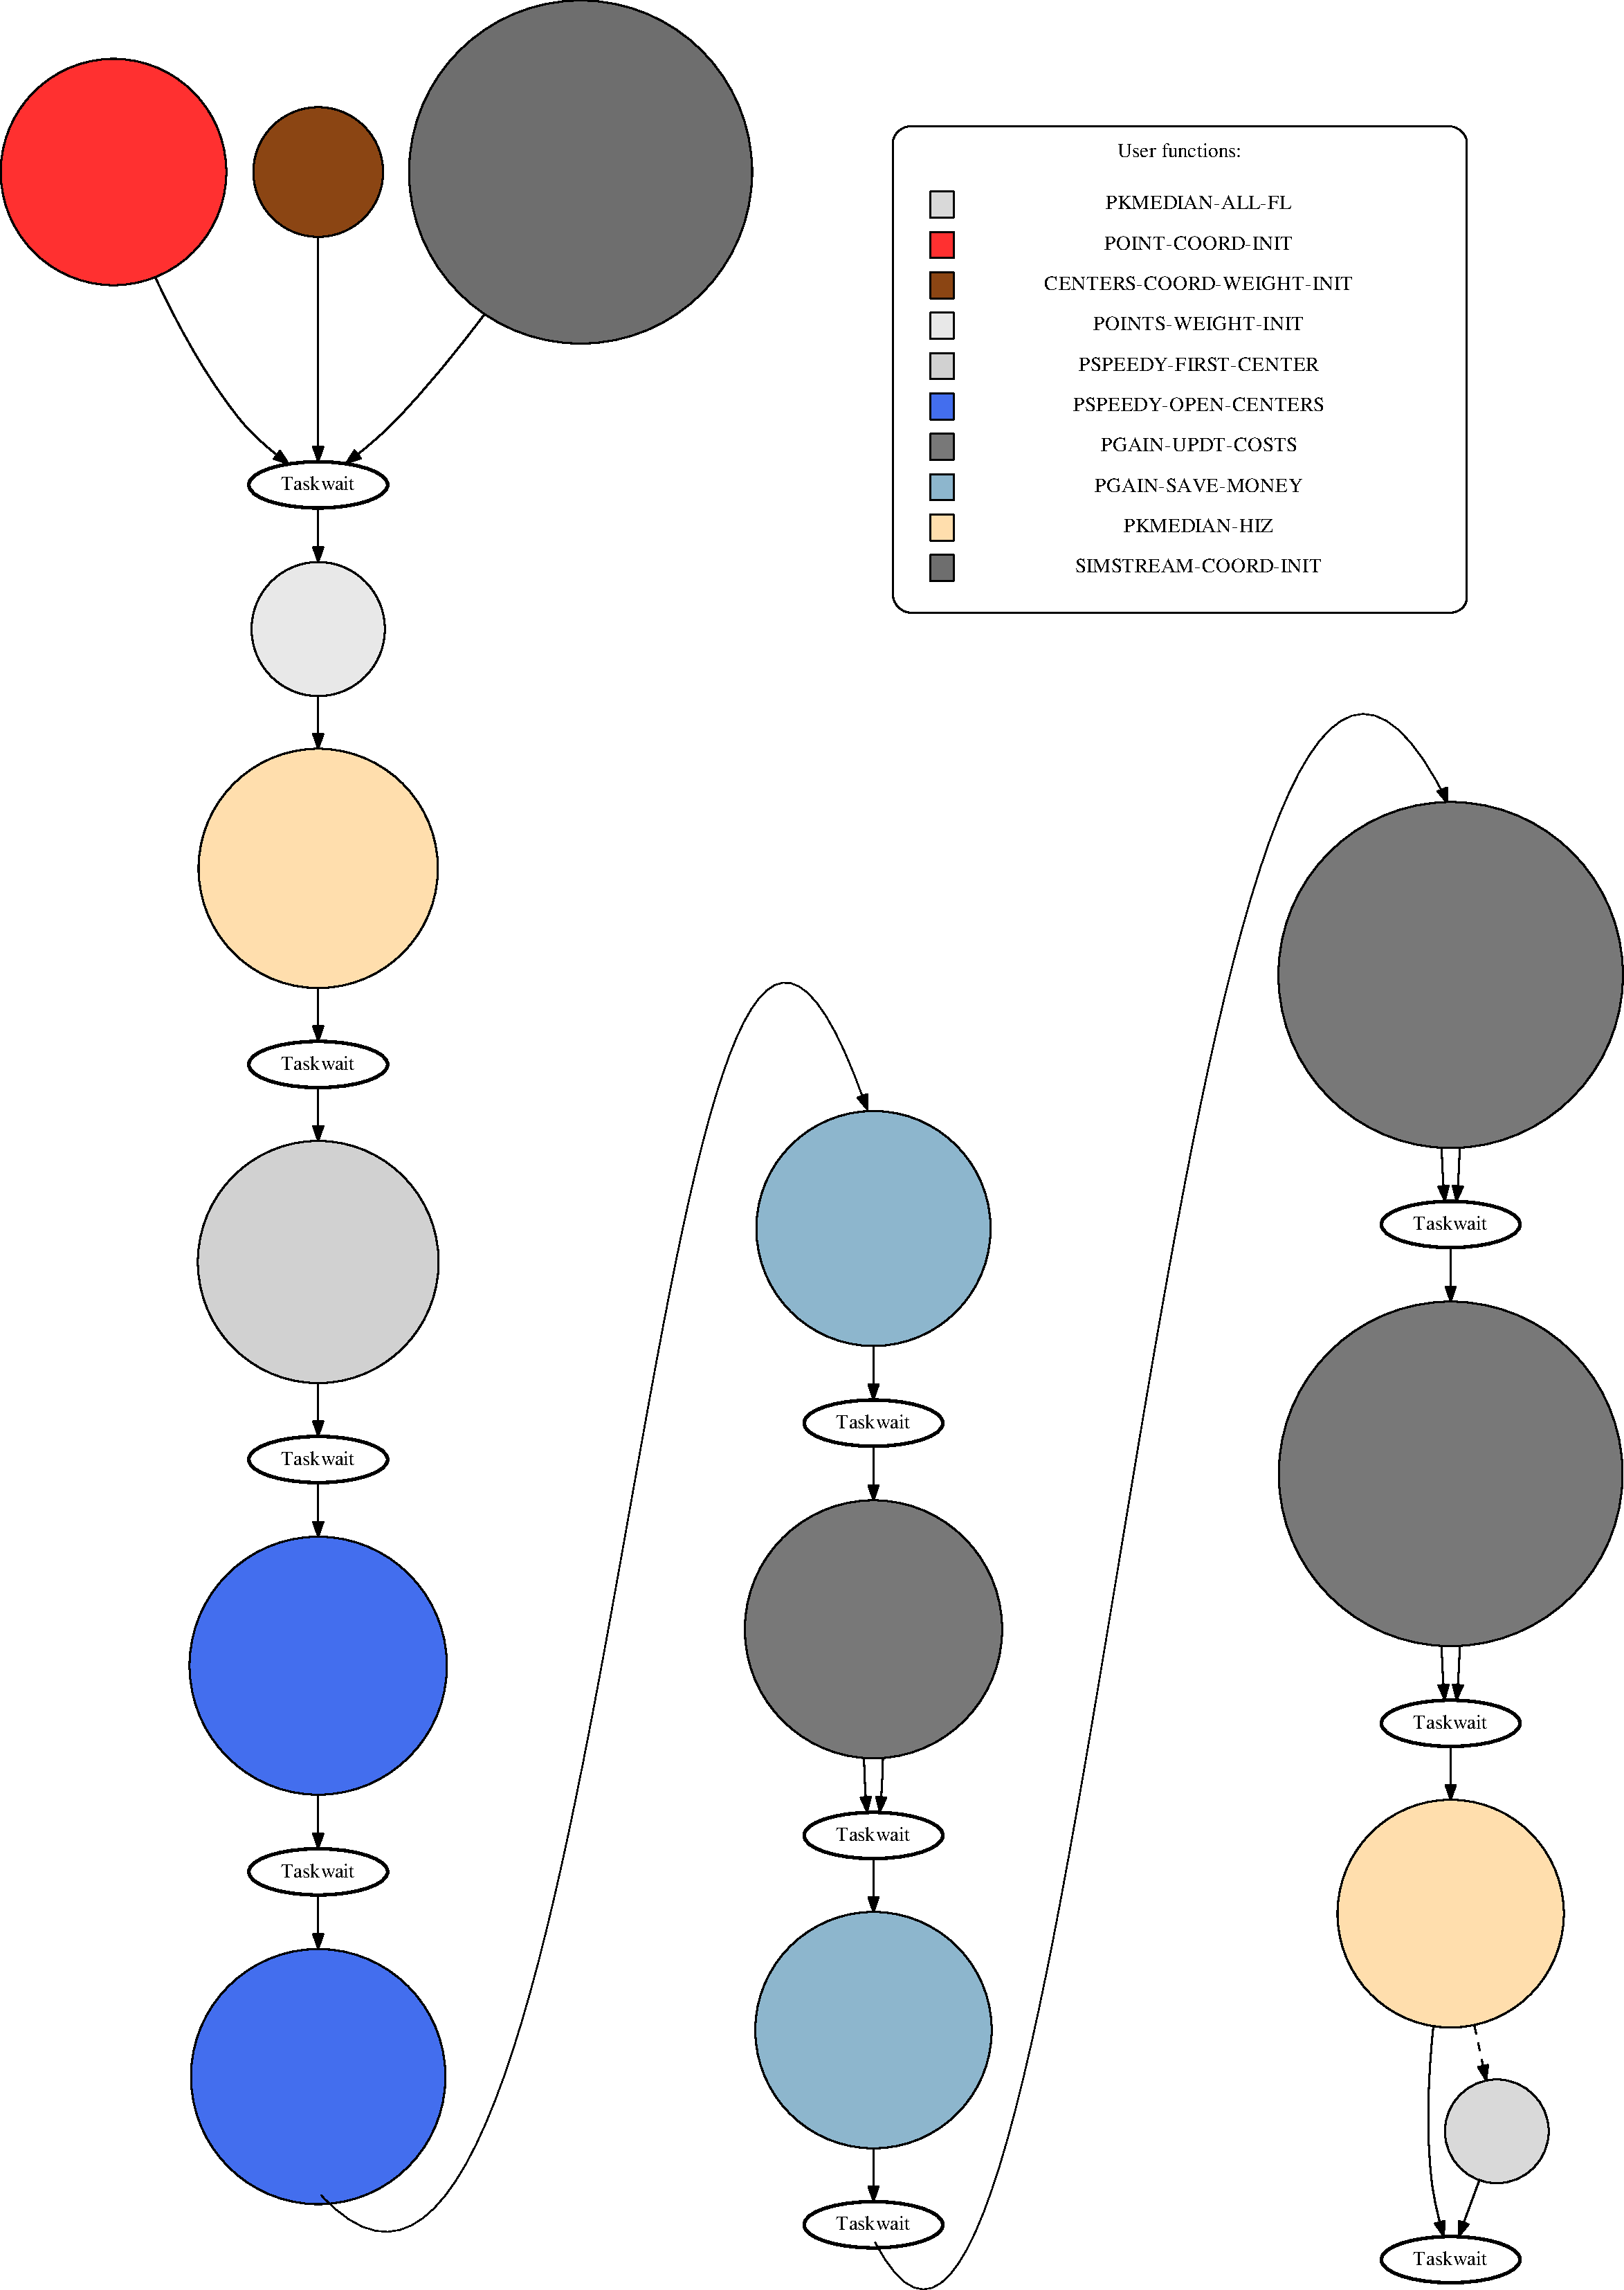
\includegraphics[width=.6\columnwidth]{ifcg/figures/streamcluster_taskgraph}%
	\caption{Task-graph of streamcluster application.  Edges represent data dependencies among
tasks.}
	\label{fig:streamcluster_tg}%
	\vspace{.5cm}
\end{figure}



\paragraph{\textit{Task-based}}
In our implementation we taskify each iteration. We do not use any dataflow relations in this application, and resolve to 
adopt the locking and barrier synchronization used in the original OpenMP version.
The barrier synchronization is shown in the task graph in figure \ref{fig:freqmine_tg}.

\paragraph{\textbf{Streamcluster}}
Streamcluster is a kernel that solves the online clustering problem. 
It takes a stream of points and then groups them in a predetermined number of clusters with their respective centers.  


\paragraph{\textit{Pthreads}}
Up to 90\% of total execution time is spent in function \texttt{pgain}, 
computing whether opening a new center is advantageous or not.  For every 
new point, function \texttt{pgain} calculates the cost of making it a new center by reassigning some points to it and 
comparing it to the minimum distance $d(x,y) = |{x-y}|^2$ between all points $x$ and $y$.
The result is accepted if found to favor the new center.  Data points are statically partitioned by a given block 
size, which determines the level of parallelism in the application. In the Pthreads version this is equal to the number of
threads. 

\paragraph{\textit{Task-based}}
In our implementation we follow a different decomposition strategy, making the number of tasks independent
of the number of partitions.   
Barriers are employed to synchronize accesses
to a partition in both Pthreads and the task-based implementation. 
In the case of Pthreads, an additional user 
implemented library is used for the barriers. 
This library is not required in the case of the OmpSs implementation, as 
the runtime already has a generic barrier implementation.
A task graph of our task-based implementation and the dependencies among tasks is shown in figure \ref{fig:streamcluster_tg}

\paragraph{\textbf{Swaptions}}
Economics application that uses the Heath-Jarrow-Morton (HJM)\cite{RePEc:ecm:emetrp:v:60:y:1992:i:1:p:77-105} for pricing of a portfolio of swaptions. To calculate prices it employs the Monte Carlo simulation.

\begin{figure}[ht!]%
	\center
	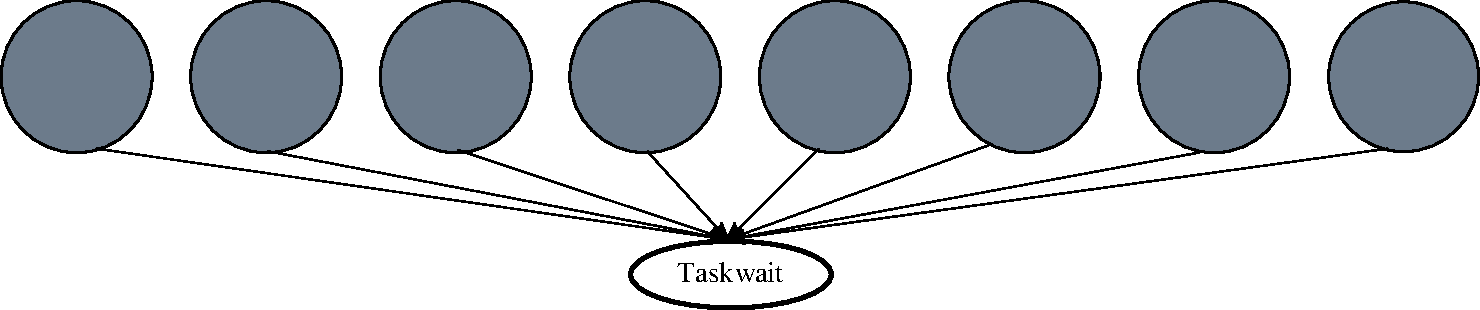
\includegraphics[width=.8\columnwidth]{ifcg/figures/swaptions_taskgraph}%
	\caption{Task-graph of swaptions application.}
	\label{fig:swaptions_tg}%
	\vspace{.5cm}
\end{figure}


\paragraph{\textit{Pthreads}}
The application stores the portfolio into an array. In the Pthreads version, this array is divided by the number of available threads, each thread working on its own part of the array. 

\paragraph{\textit{Task-based}}
We use the exact same strategy, where each task works on a part of the array.  No data dependencies exist between the tasks.
Figure \ref{fig:swaptions_tg} shows the corresponding task graph for the swaptions application.  No dependencies exist between tasks,
synchronization is only achieved through barriers.
%\paragraph{\textbf{x264}}
%An AVC (Advanced Video Coding) video encoder, based on the ITU-T H.264 standard~\cite{H.2642007}.
%It improves over previous video encoding standards at the expense of significantly increased 
%encoding and decoding time.


%The parallel version of x264 extracts parallelism by processing different frames concurrenlty. Initially frames are split in smaller 
%macroblocks of 16x16 pixels.  These macroblocks are processed by a pipeline with a number of stages equal to the number of frames.
%The stages are: \texttt{Read\_frame}, which reads input frames, \texttt{Analyse\_frame}, which creates data dependencies among macroblocks,
%\texttt{Encode\_frame}, which is the encoding state and \texttt{Write\_frame} which writes the encoded frames to the output file.


%The task-based implementation does not use the macroblocks. Instead
%it works on whole frames.  We use two different task types, each spawned for each frame.  The first reads the frame and the second performs the
%three other pipeline stages.  The pipeline stages are synchronized using shared variables. 
 
